Combining fuzz testing with symbolic execution has been proved to be a promising approach to improve the testing performance. Driller, which is built on top of Angr symbolic execution engine and AFL fuzzing engine, has attempted to leverage symbolic execution to assist fuzz testing in exploring as many as paths. And its performance in the CGC challenge has been the great supporting evidence for this combinatorial testing approach. 

We also leveraged this approach in our method and enhanced it by introducing two improvements. In our method, symbolic loops (loop boundary depends on symbolic data) have been carefully taken care by Symbolic Loop Bucket (SLB). Meanwhile, we introduced a novel method called Lazy Symbolic Pointer (LSP) to handle symbolic pointers. In the following sections, the basic workflow of this combinatorial testing approach will be introduced briefly first. Then, the details of SLB and LSP will be discussed.

\subsection{Assist fuzz testing with concolic execution}
The basic framework of this combinatorial testing approach is shown in Figure~\ref{s2e-assist}. The fuzzing engine performs evolutionary mutation testing and shares the internal data, which is used to record the path information (such as the bitmap in AFL), with the symbolic execution engine. When the fuzzing engine starts to be saturated, the current seed file will be sent to symbolic execution engine to uncover more new paths. Unlike traditional symbolic execution, the seed file is used to execute as concolic execution (as shown the red execution path). Then, based on the shared internal bitmap, the symbolic execution can determine which branch has not been covered yet (the yellow branch in the figure). For these uncovered branches, the symbolic execution engine will invoke the constraint solver to generate a corresponding test case. Under this execution mode, the ``path explosion'' problem will be avoided to a large extent. And all the generated new seed files will be feed into the test case queue of the fuzzing engine.

Compared with using symbolic execution and fuzz testing separately, this combinatorial approach can take the advantages of both methods and mitigate the ``path explosion'' problem by this scale controllable concolic execution. Meanwhile, the fuzzing engine will not be saturated in a short time with the assistance of the fresh test cases generated by concolic execution.

\begin{figure}
\centering
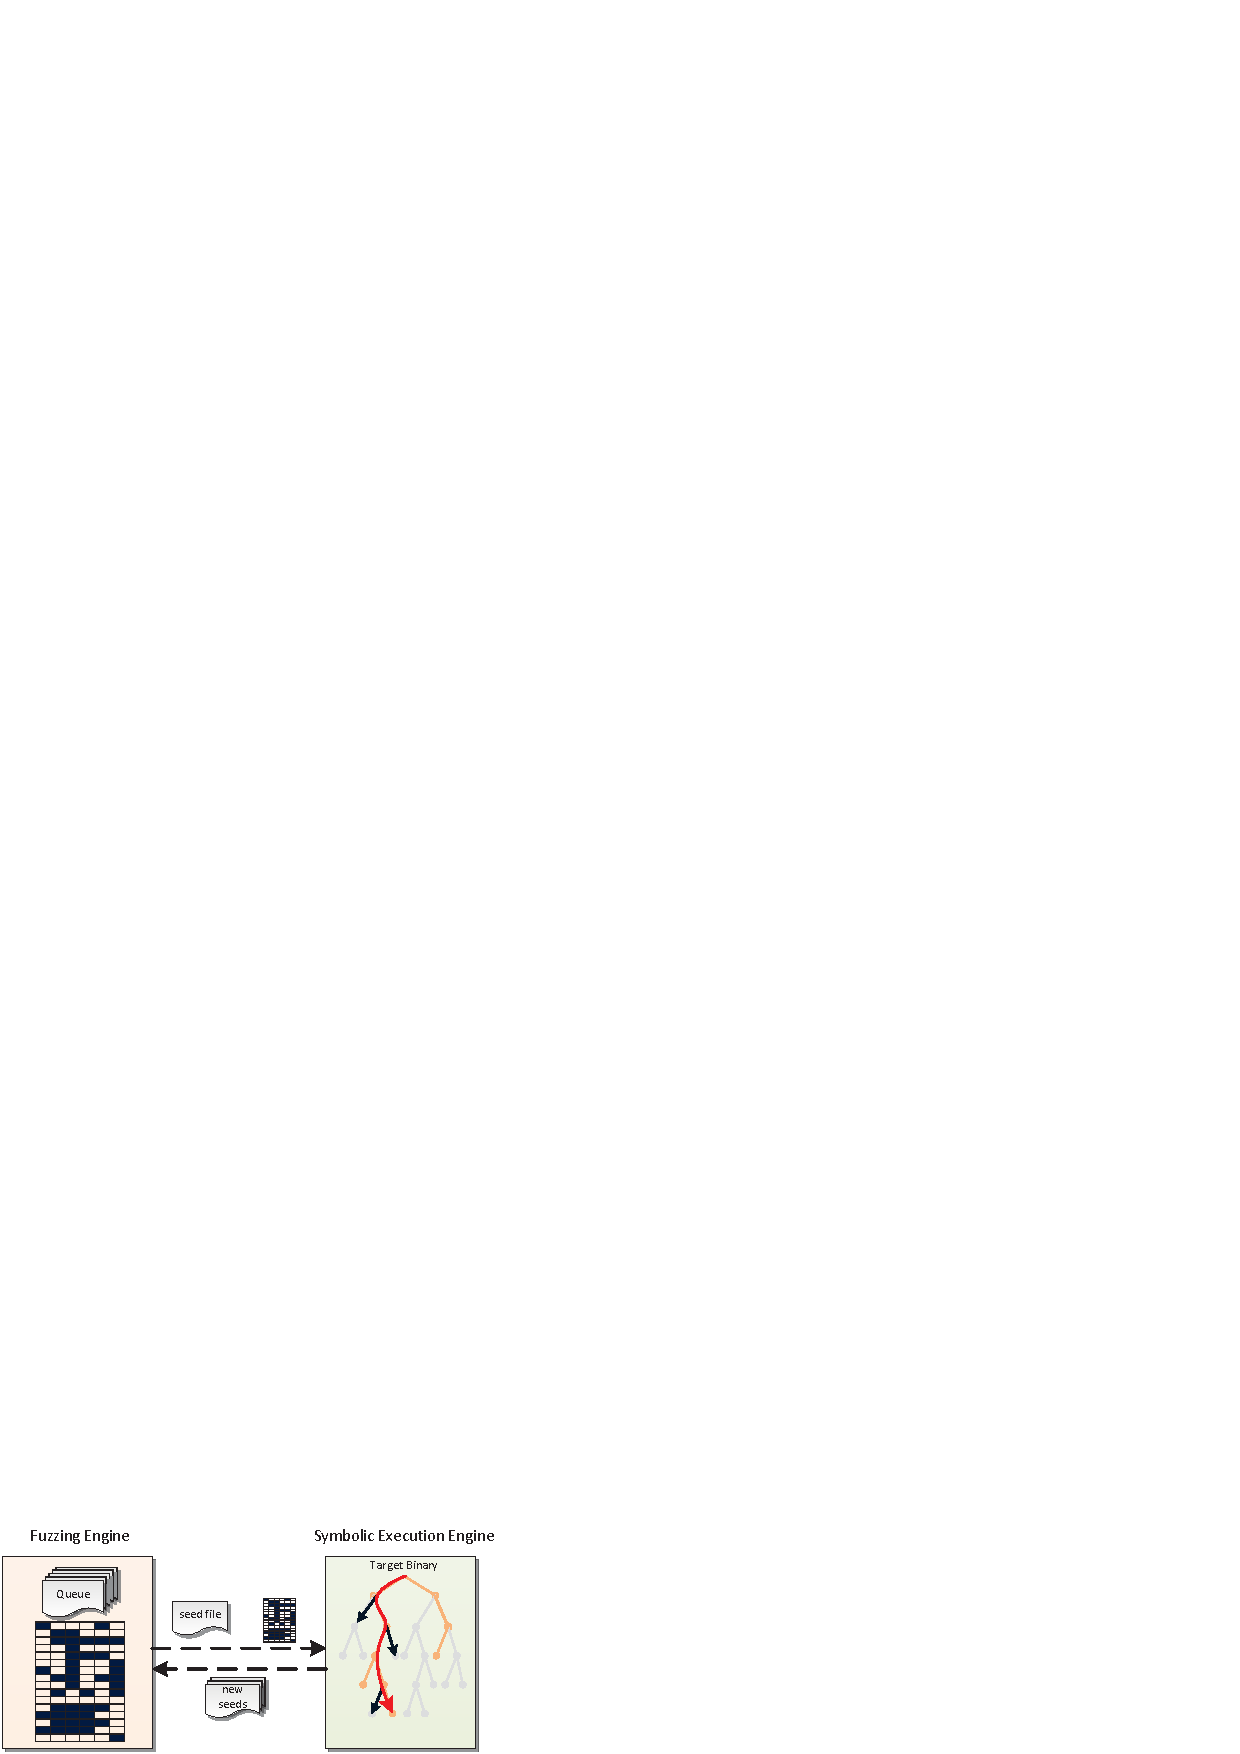
\includegraphics[width=0.7\textwidth]{figures/s2e-assist.pdf} 
\caption{Assist fuzz testing with concolic execution.}\label{s2e-assist}
\end{figure}


\subsection{Symbolic Loop Buckets}
Symbolic loop, whose loop control variable depends on symbolic data, will cause serious ``path explosion'' problem as its loop times will range from 0 to infinite for the worst case. So the symbolic loops have to be carefully handled to avoid getting stuck at the loop spot. AFL utilizes \emph{Loop Bucket} mechanism to solve this problem. It groups the loop times into different buckets, i.e. [1, 2, 3, 4-7, 8-15, 16-31, 32-127, 128+]. Only changes happened between different buckets will be regarded as new behaviors. Based on this idea in fuzz testing, we proposed a Symbolic Loop Bucket (SLB) to handle the symbolic loop bucket. The algorithm of SLB is described in Algorithm~\ref{SLB}.

Loops are extracted from the target program by static analysis. These loops will be configured to symbolic execution engine to help it recognize loops in runtime. All the symbolic loops can be distinguished from the others by checking the loop exit condition from the symbolic execution engine (Line 2$\sim$3). For the edges belong to symbolic loop, the uncovered loop bucket for this loop will be obtained by analyzing the Bitmap mentioned before (Line 5). State forking is disabled in already covered loop buckets, and once an uncovered bucket is reached, the corresponding test case will be generated and then this uncovered bucket will be removed from the uncovered loop buckets to avoid generating multiple test cases (Line 6$\sim$17). This can make sure that all the loop buckets will be covered without coming across with the ``path explosion'' problem.

\begin{algorithm}
  \caption{Symbolic Loop Bucket}
  \label{SLB}
  \KwIn{Configured Loops $L$, Current Edge $CE$ and Bitmap $B_p$}  
  \If{not $IsaLoopCycleEdge(L,CE)$ or not $IsaSymLoop(CE)$}
  {
    return;
  }
  $loopTimes$ = 1\;
  $UBs$ = $ParseUncoveredBuckets(B_p)$\;
  \While{TRUE}
  {
    \ForEach{$ub$ in $UBs$}
    {
      \If{$loopTimes$ within $ub$}
      {
        $GenerateTestcase()$\;
        $UBs$.$remove(ub)$\;
      }
    }
    \eIf{$UBs$ is $null$}
    {
      break\;
    }{
      $ExecuteOneCycle()$\;
      $loopTimes += 1$\;
    }
  }
\end{algorithm}  

\subsection{Lazy Symbolic Pointer}
The motivated code snippet in Listing~\ref{RE-LSP} shows the basic symbolic pointer problem in symbolic execution. The EAX register in line 6 is a symbolic data that derived from the input file. And text\_char is a concrete const Boolean Array that represents the whether the EAX value is an ASCII text. Then based on the returned value from text\_char, the code will perform some further process (Line 8$\sim$10). Because the EAX in Line 6 is marked as symbolic, so it will lead to the symbolic pointer problem as it can point to multiple addresses.


When given a symbolic pointer, based on different memory models, different handle process can be taken. For example, in full symbolic memory model, each possible value of this pointer will fork a corresponding state. There also exists a strategy namely address concretization which will concretize the pointer to a single specific address. Obviously, the full symbolic memory model will raise the serious state explosion and the address concretization may lose some interesting paths. To mitigate the scalability problems of full symbolic memory model and the loss of interesting paths of address concretization, a partial symbolic memory model has been to make a trade-off in recent years. The partial symbolic memory model tries to concretize all symbolic pointer write operation and treats all symbolic pointer read operation as full symbolic memory model. 

The lazy forking strategy in S2E is also leveraged to ease the problem along with the large number of states forked from symbolic pointer read operation in partial symbolic memory model. Lazy forking is utilized to avoid maintaining expensive symbolic pointers in concolic execution. For example, for the instruction in Line 6 in Listing~\ref{RE-LSP}, suppose EAX is read from the input file and its concrete value is 0x41. Then when the concolic execution engine executes to this statement, it will try to fork the current state with a hard constraint which can be expressed as ``$EAX == 0x41$''. Unlike the other memory models, the engine will not fork all the possible value for EAX but only add the soft constraint of ``$EAX \neq 0x41$'' to the other forked state, which will reduce the number of state to a large extent. 

\lstinputlisting[label={RE-LSP}, language=nasm,style=nasm,caption={A real-world binary code that contains symbolic pointer dereference.}]{codes/real-eaxmple-LSP.asm}

While because of the hard constraint, the state forking at Line 10 will fail for the original state which means some soundness paths will not be covered by this state. As the objective of concolic execution is to assist fuzz testing to uncover more paths as soon as possible, so this will bring some performance loss. To mitigate this problem, we introduced a method called Lazy Symbolic Pointer which is built on top of partial symbolic memory model and lazy forking. The detailed algorithm of LSP is shown in Algorithm~\ref{LSP}.
\begin{algorithm} [htpd]
  \caption{Lazy Symbolic Pointer}
  \label{LSP}
  \KwIn{Current State $S$, Pending States $S_P$ and Hard Constraint $C_H$}
  \KwOut{Testcase $t_{lsp}$ if success}
  $C_F = getFailedCondition()$\;
  $offs = S.getInputOffset(C_F)$\;
  \If{$S_P.find(offs) == S_P.end()$}
  {
    return $null$\;
  }
  $Conditions = S.getRelateConditions(offs).strip(C_H)$\;
  \ForEach{$s_p$ in $S_P.find(offs)$}
  {
    $s_{tmp} = s_p.clone()$\;
    $s_{tmp}.addConstraint(Conditions)$\;
    $s_{tmp}.addConstraint(C_F)$\;
    $(success, t_lsp) = s_{tmp}.generateTestcase()$\;
    \eIf{$success$}
    {
      return $t_{lsp}$;
    } {
      continue;
    }
  }
  return $null$\;
\end{algorithm}  

When performing lazy forking, all the states whose path constraints contain the soft constraints will be collected into the \emph{Pending States}. And the pending states are grouped by the input offsets that affect the corresponding soft constraint (Line 6\&7). For the soft constraint that may be affected by more than one input offsets, the pending state will be collected to the groups of all the offsets in the constraint. For example, as the soft constraint ``Not (Eq (ReadLSB w32 0x10 symbolic\_input, 0x41))'' is affected by four bytes (i.e. 0x10, 0x11, 0x12 and 0x13), so the pending state will be appended to the groups indexed by 0x10, 0x11, 0x12 and 0x13. 

Then when the symbolic execution engine fails to fork at the branch that depends on soft constraints, such as the branch at line 10 in Listing~\ref{RE-LSP}, the failed condition will be inspected to extract the input offsets that affect this branch (Line 10\&11). LSP ignores the case that the reason of fork failure does not result from the lazy forking (Line 12\&13). For every offset that affects the failed condition, we extract all the related conditions in path constraints except for the hard constraint (Line 14), and then these conditions will be added to the pending states that related to the input offset to generate test cases (Line 15$\sim$18). 

% TODO: Add a real example, or it is hard to understand %

Based on this algorithm, we can generate at least one new test case that satisfies the failed condition where the fork failure occurs because of lazy forking. But we still need to prove this test case will steer the program to execute the same path with the original state and then covers the branch that fails in the original state. A quick execution consistency proven is explained as follows:

Let $P_A$ is the execution path of a state $A$:
\begin{center}
$P_A = (B_0,T) \rightarrow (B_1,T) \rightarrow (B_2,F) \rightarrow (B_3,T)
\rightarrow (B_4,F) \rightarrow (B_5,F) \rightarrow (B_6,F) \rightarrow (B_u,T)$
\end{center}

\noindent where $B_n$ refers to the $n-th$ branch. $T/F$ means state $A$ takes the \emph{True/False} branch and $B_u$ denotes the branch where the forking fails because of the extra hard constraint. Assume that hard constraint is $var==0xAB$ which is originated from the lazy forking from $B_1$, and the conditions at $B_3$ and $B_5$ are also affected by $var$.

Suppose state $B$ is the corresponding pending state forked from $B_1$, and then, according to the LSP algorithm in Listing~\ref{LSP}, when state $A$ raises a fork failure at branch $B_u$, all the related constraints except the hard constraint will be added to state $B$. After that, the path constraint of state $B$ will be:
\begin{center}
$PC_B = \displaystyle ^\neg CB_u \cap ^\neg CB_1 \cap \bigcap\limits_{i=0,i \neq 1}^{6} CB_i$
\end{center}
\noindent where the $CB_i$ denotes the path condition at branch $B_i$. We need to prove the following formula.
\begin{center}
$\mathbb{Z} = \{var\arrowvert PC_B(var) = True\} \neq \emptyset$
\end{center}

As there are only two branches before $B_u$ that depend on $var$, so the expression $PC_B$ can be simplified to:
\begin{center}
$PC_B = ^\neg CB_u \cap ^\neg CB_1 \cap CB_3 \cap CB_5$
\end{center}

There are two possible cases for $CB_3 \cap CB_5$:
\begin{center}
case1: $CB_3 \cap CB_5 = (var == 0xAB)$

case2: $CB_3 \cap CB_5 \neq (var == 0xAB)$
\end{center}

Under the first case, the path to $B_u$ is only feasible when $var$ equals to 0xAB. So the edge $(B_u, F)$ will never be satisfied (i.e. \emph{dead code}) because $(var == 0xAB) \subseteq CB_u$. For the second case, there must be at least one feasible solution for $var$ that satisfies with the soft constraint $^\neg CB_1$, so $^\neg CB_1 \cap \bigcap_{i=0,i \neq 1}^{6} CB_i$ can be evaluated to $True$ for some specified values of $var$. This has proved that there must be at least one test case under $PC_B$ that can steer the program to the forking failure point $B_u$.

Similarly, for branch condition $B_u$, there are also two possible cases:
\begin{center}
case1: $\displaystyle ^\neg CB_1 \cap \bigcap\limits_{i=0,i\neq 1}^6 CB_i \subseteq CB_u$

case2: $\displaystyle ^\neg CB_1 \cap \bigcap\limits_{i=0,i\neq 1}^6 CB_i \nsubseteq CB_u$
\end{center}

The first case, which can also be expressed as $^\neg CB_u \cap ^\neg CB_1 \cap \bigcap_{i=0,i\neq 1}^6 CB_i = \emptyset$, is the case of \emph{dead code}. And the second case can be transformed into:
\begin{center}
$\displaystyle ^\neg CB_u \cap ^\neg CB_1 \cap \bigcap\limits_{i=0,i\neq 1}^6 CB_i \neq \emptyset \implies \mathbb{Z} = \{var\arrowvert PC_B(var) = True\} \neq \emptyset$
\end{center}

\noindent which means there must be at least one feasible value that satisfies with the false branch of $B_u$. So above all, we can draw a conclusion that our \emph{LSP} algorithm can keep the execution consistency when $(B_u, F)$ is not dead code.